\section{Method}
\label{app:all_method_details}

\subsection{Model details}
\label{app:experiment_and_model_details}

\begin{figure}[t]
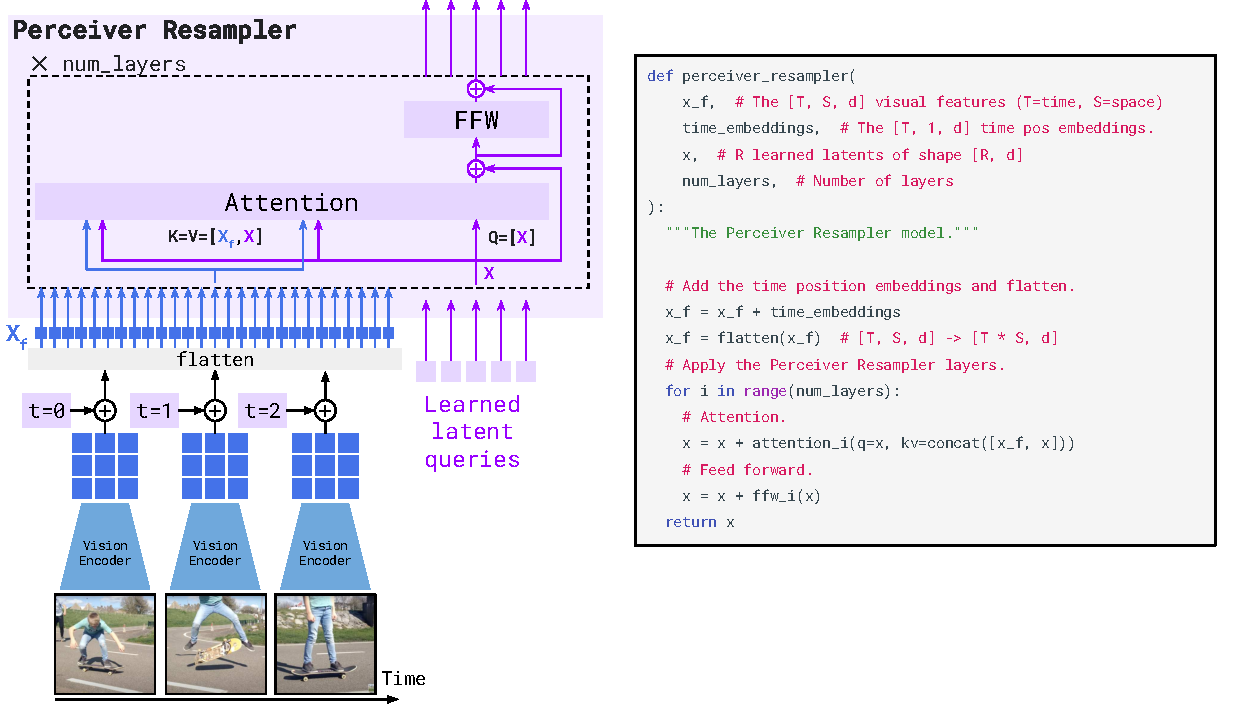
\includegraphics[width=\linewidth]{figures/fig3_resampler.pdf}
\centering
\caption{\capfontsize{} \textbf{The Perceiver Resampler} module maps a \emph{variable} size grid of spatio-temporal visual features output by the Vision Encoder to a \emph{fixed} number of output tokens (five in the figure), independently from the input image resolution or the number of input video frames.
This transformer has a set of learned latent vectors as queries, and the keys and values are a concatenation of the spatio-temporal visual features with the learned latent vectors.}
\label{fig:transformer_resampler}
\end{figure}




\subsubsection{Perceiver Resampler}
\label{app:transformer_resampler}
Expanding on our brief description in Section~\maintoappref{sec:transformer_resampler},
Figure~\ref{fig:transformer_resampler} provides an illustration of our Perceiver Resampler processing an example video, together with pseudo-code.
Our Perceiver Resampler is similar in spirit to the Perceiver models proposed by~\citet{jaegle2021perceiver}.
We learn a predefined number of latent input queries, and cross-attend to the flattened visual features $X_f$.
These visual features $X_f$ are obtained by first adding a learnt temporal position encoding to each feature within a given video frame (an image being considered as a single-frame video).
Note that we only use temporal encodings and no explicit spatial grid position encodings;
we did not observe improvements from the latter.
This rationale behind is likely that CNNs, such as our NFNet encoder, are known to implicitly include spatial information channel-wise~\citep{islam2021global}.
The visual features are then flattened and concatenated as illustrated in Figure~\ref{fig:transformer_resampler}.
The number of output tokens of the Perceiver Resampler is equal to the number of learnt latent queries.
Unlike in DETR and Perceiver, the keys and values computed from the learnt latents are concatenated to the keys and values obtained from $X_f$, which we found to perform slightly better.


\subsubsection{\textsc{gated xattn-dense} details}
\label{app:xattn_dense}
We provide in Figure~\ref{fig:xattn_dense} an illustration of a \textsc{gated xattn-dense} block and how it connects to a frozen LM block, together with pseudo-code.

\begin{figure}[t] 
 \captionsetup[subfigure]{justification=centering}
  \subfloat[Attention tanh gating]{%
    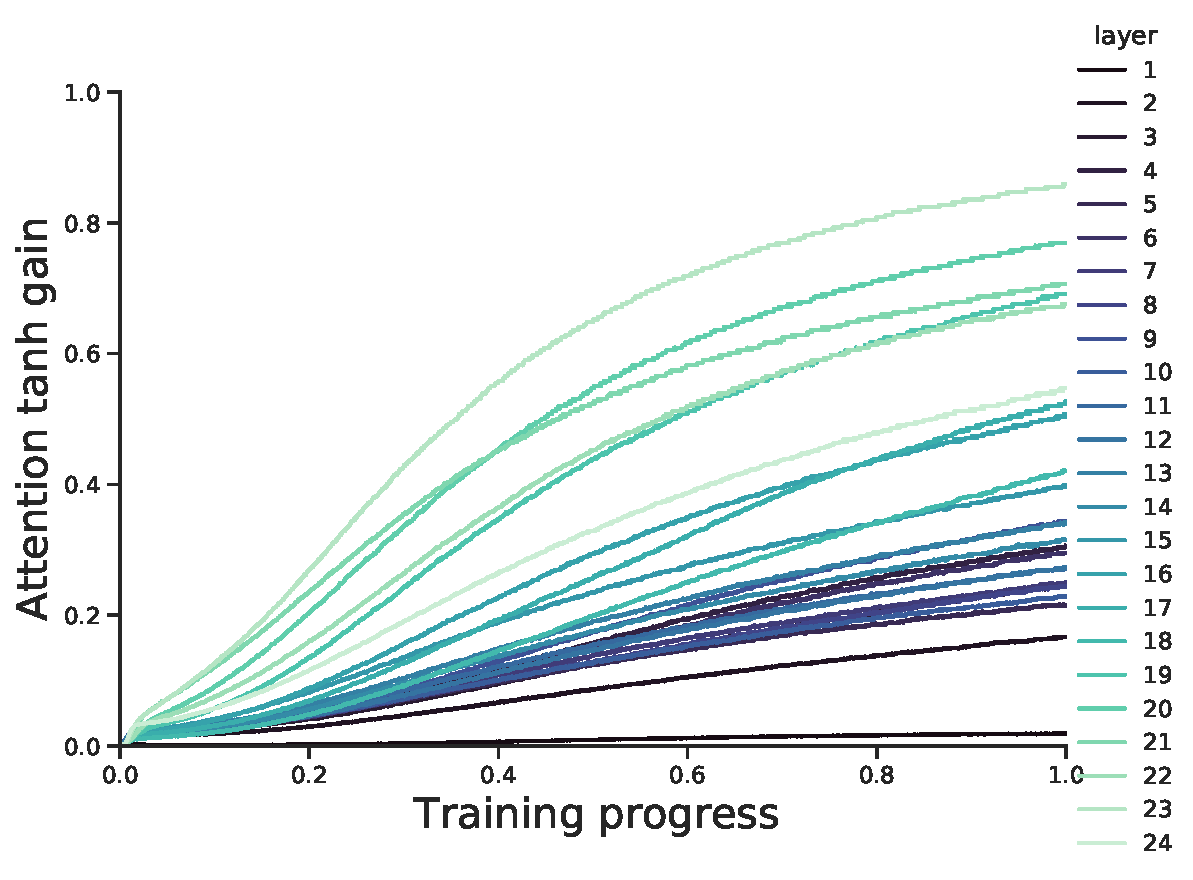
\includegraphics[width=0.47\textwidth]{figures/attn_gain.pdf}
  } 
  \hfill 
  \subfloat[FFW tanh gating.]{%
    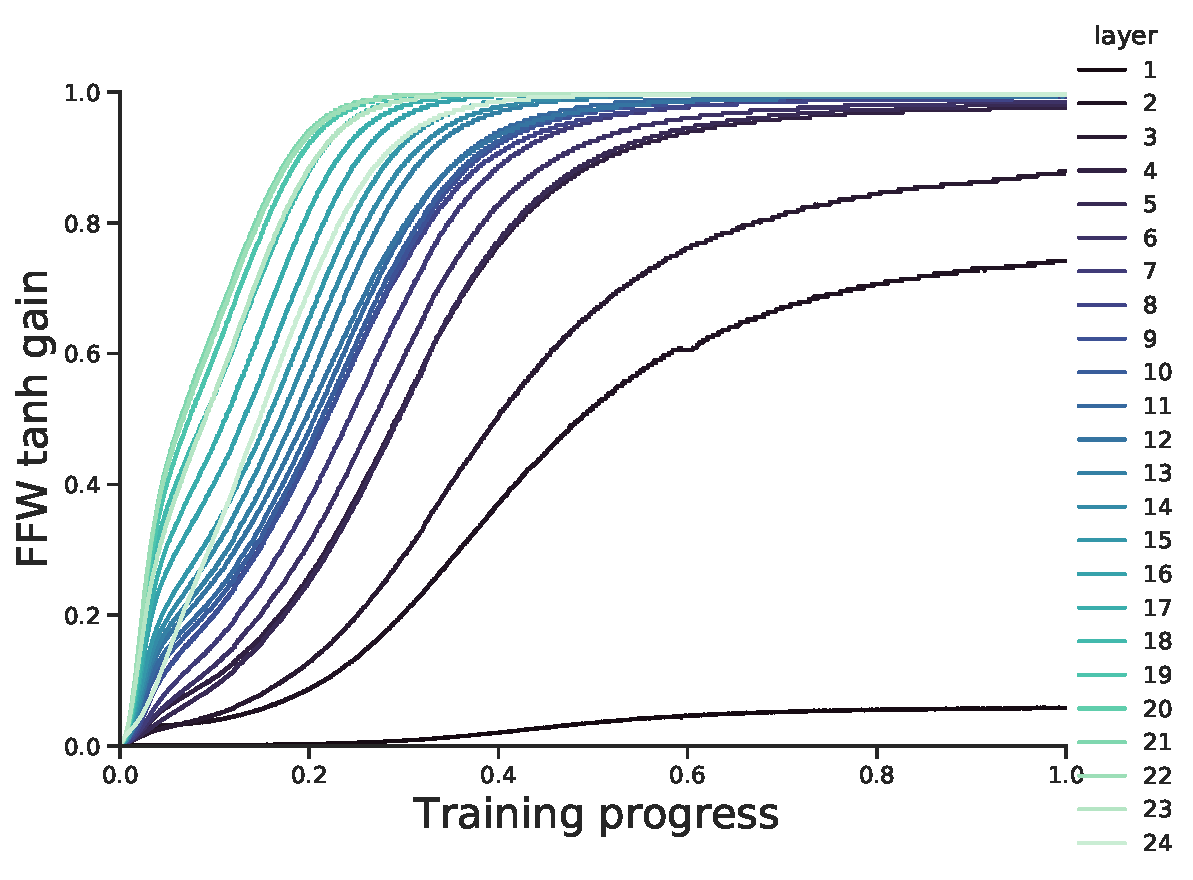
\includegraphics[width=0.47\textwidth]{figures/ffw_gain.pdf}
  } 
  \caption{\capfontsize{} Evolution of the absolute value of the tanh gating at different layers of \base{}.
  } 
  \label{fig:tanh_gating_evolution}
\end{figure}


We also plot in Figure~\ref{fig:tanh_gating_evolution} the evolution of the absolute value of the $\tanh$ gating values as a function of training progress (from $0\%$ to $100\%$) at different layers of the LM stack for the \base{} model composed of 24 LM layers.
All layers of the frozen LM stack seem to utilize the visual information as the $\tanh$ gating absolute values quickly grow in absolute value from their 0 initializations.
We also note that the absolute values seem to grow with the depth.
However, it is difficult to draw strong conclusions from this observation: the scale of the activations before gating may also vary with depth.
Future work is required to better understand the effect of these added layers on the optimization dynamics and on the model itself.



\subsubsection{Multi-visual input support}
\label{app:multi-visual-details}

We illustrate in Figure~\ref{fig:xattn_multi_im} the masking approach we use to limit the number of visual tokens that a certain text token sees.
We also formalize our notation for the interleaved sequences of images/videos and text.

\begin{figure}[t]
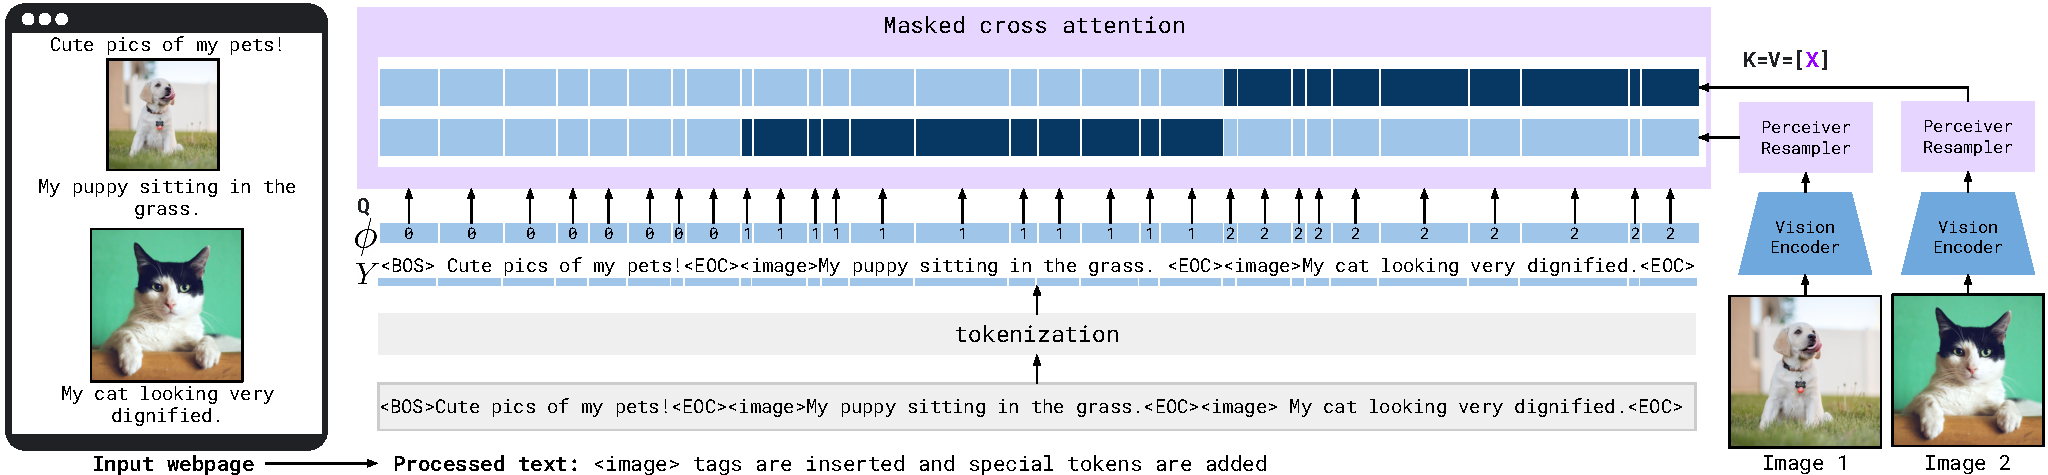
\includegraphics[width=\linewidth]{figures/fig5_multi_im_att.pdf}
\centering
\caption{\capfontsize{} \textbf{Interleaved visual data and text support.} 
Given text interleaved with images/videos, e.g. coming from a webpage, we first process the text by inserting \texttt{<image>} tags at the locations of the visual data in the text as well as special tokens (\texttt{<BOS>} for ``beginning of sequence'' or \texttt{<EOC>} for ``end of chunk'').
Images are processed independently by the Vision Encoder and Perceiver Resampler to extract visual tokens.
At a given text token, the model only cross-attends to the visual tokens corresponding to the last preceding image/video. 
$\phi$ indicates which image/video a text token can attend or $0$ when no image/video is preceding.
In practice, this selective cross-attention is achieved through masking -- illustrated here with the dark blue entries (unmasked/visible) and light blue entries (masked).
}
\label{fig:xattn_multi_im}
\end{figure}

\textbf{Interleaved sequences of visual data and text.}
We consider interleaved image/video and text examples: each example holds a sequence of text $y$, a sequence of images/videos $x$, and the sequence of positions of the images in the text. Based on the visual data positions, we define a function $\phi: [1, L] \mapsto [0, N] $ that assigns to each text position the index of the last image/video appearing before this position (or $0$ if no visual data appears before the position). 
The function $\phi$ defines which visual inputs we consider usable to predict token $\ell$ in Equation~\eqref{eq:modeling}: the set of preceding tokens $y_{< \ell} \triangleq (y_1, \dots, y_{\ell-1})$, and the set of preceding images/videos $x_{\leq \ell} \triangleq \{ x_i | i \leq \phi(\ell) \}$.


\subsubsection{Transformer architecture}
\label{app:transformer_details}

\begin{table}[h]
\centering
\footnotesize
\begin{tabular}{@{}l|cccc|cccc|cccc@{}}
\toprule
                        & \multicolumn{4}{c|}{Perceiver Resampler} & \multicolumn{4}{c|}{\textsc{gated xattn-dense}}  & \multicolumn{4}{c}{Frozen LM} \\ 
                        & L & D & H  & Act. & L & D & H   & Act. & L & D & H  & Act. \\ \midrule
\base{}            &   6    &  1536  & 16 & Sq. ReLU &   24   &  2048  & 16 & Sq. ReLU & 24 &  2048 &  16  & GeLU    \\
\medium{}          &   6    &  1536  & 16 & Sq. ReLU &   10    &  4096  & 32 & Sq. ReLU & 40 &  4096 & 32 & GeLU   \\
\largem{}           &   6    &  1536  & 16 & Sq. ReLU &   12    &  8192  & 64 & Sq. ReLU & 80 &  8192 &  64 & GeLU \\ \bottomrule
\end{tabular}%
\vspace{1em}
\caption{Hyper-parameters for the \methodfamily{}' transformers. The hidden size of each feed-forward MLP is $4D$. \textbf{L}: number of layers, \textbf{D}: transformer hidden size, \textbf{H}: number of heads, \textbf{Act.}: FFW activation, \textbf{Sq. ReLU}: Squared ReLU~\citep{so2021primer}.
}
\label{tab:model-architecture-hyperparam}
\end{table}

We list in Table~\ref{tab:model-architecture-hyperparam} the number of layers ($L$), the hidden dimension ($D$), the number of heads ($H$), and the FFW activation (Act.) used for each transformer component of our \method{} models.
The dimension of keys and values in each configuration is given by $D/H$ (96 for the Perceiver Resampler; 128 for \textsc{gated xattn-dense} and the frozen LM),
and the hidden dimension of each feed-forward MLP is $4D$.
Note that the frozen LM was trained with the GeLU activation~\citep{hendrycks2016gaussian}, while the remaining trainable transformer layers use the Squared ReLU activation~\citep{so2021primer}, which we found to outperform GeLU.




\subsection{In-context few-shot evaluation details}
\label{app:in_context_eval_details}

\begin{figure}[t]
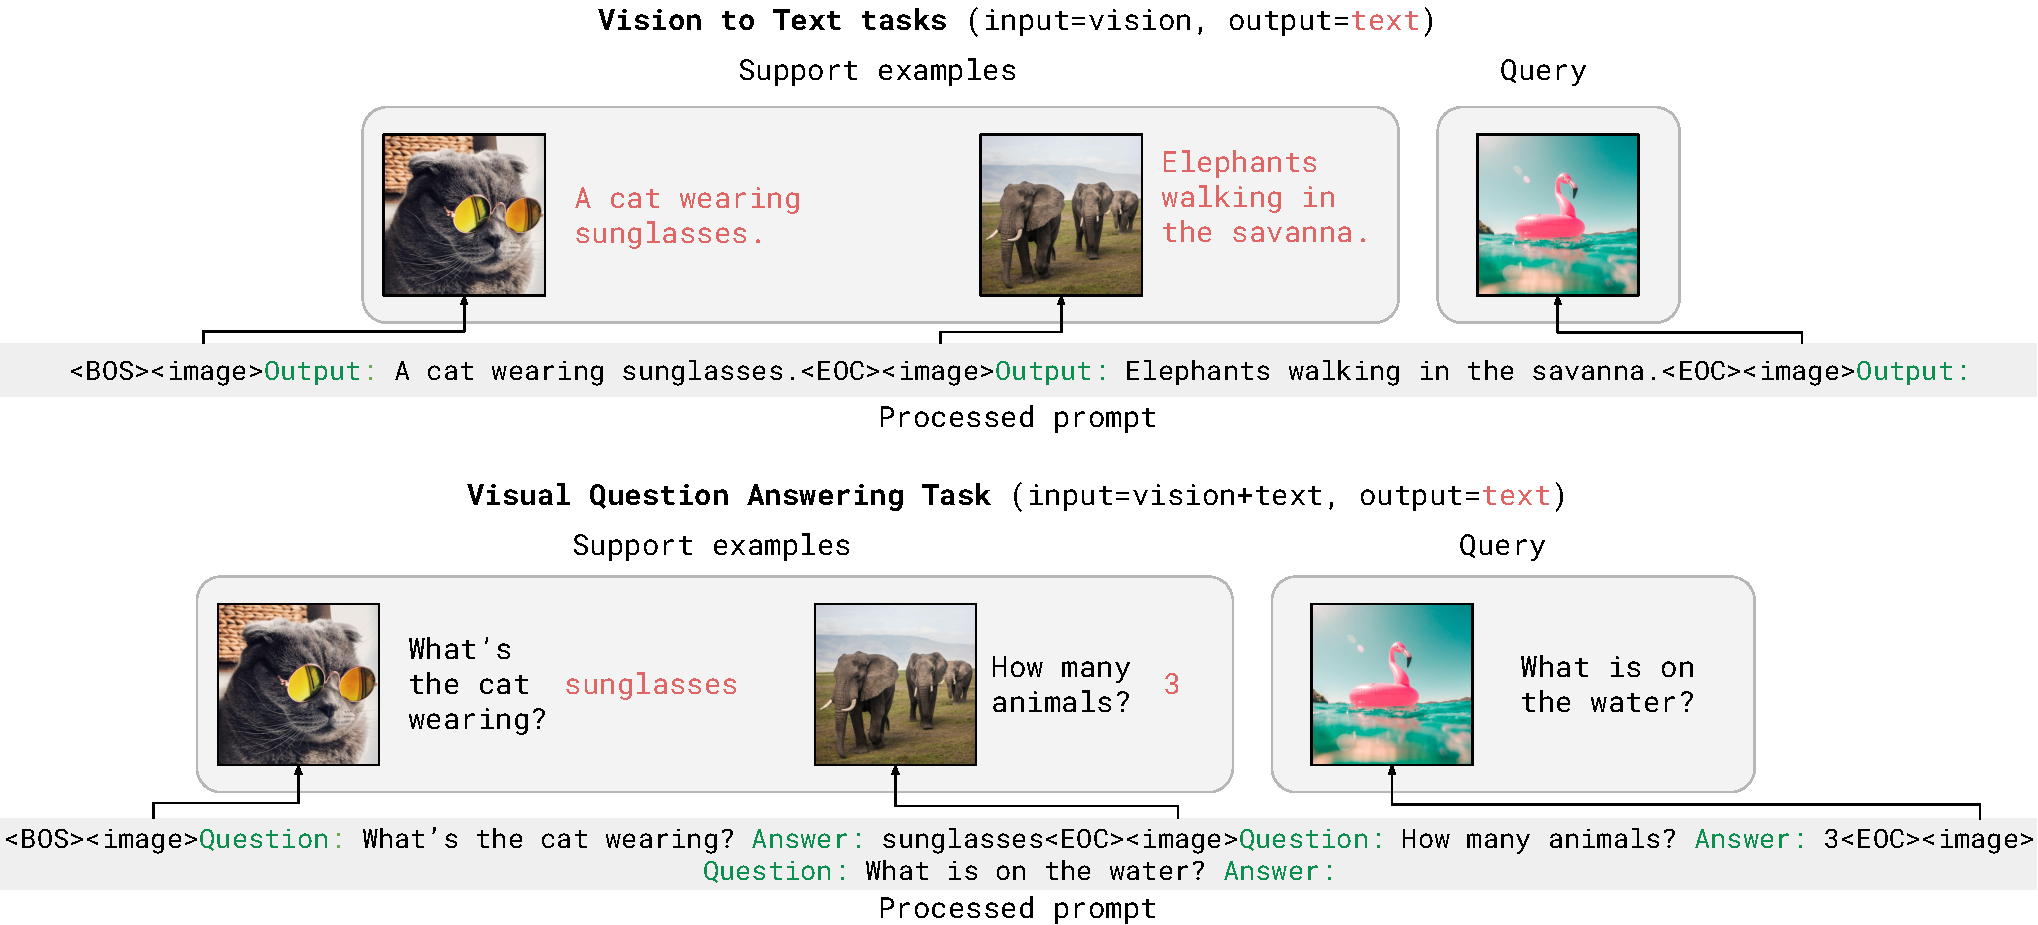
\includegraphics[width=\linewidth]{figures/fig_fewshot_prompt.pdf}
\centering
\caption{\capfontsize{} \textbf{Few-shot interleaved prompt generation.}
Given some task-specific few-shot examples (a.k.a.  support examples) and a query for which~\method{} should make a prediction, we build the prompt by interleaving images with their corresponding texts.
We introduce some formatting to do this, prepending
``\texttt{\color{greencode}Output:}'' to the expected response for all vision-to-text tasks or prompting in the format ``\texttt{\color{greencode}Question:~\{question\}\color{greencode}~Answer:~\{answer\}}'' for visual question-answering tasks.
}
\label{fig:fewshot_prompt}
\end{figure}


\paragraph{In-context learning with \method{} models.}
We evaluate the ability of our models to rapidly adapt to new tasks using in-context learning, following an analogous approach to the one used in GPT-3~\citep{gpt3}.
In detail, we are given a set of support examples in the form of $(image, text)$ or $(video, text)$ (where the $image$ or $video$ is the input visual and the $text$ is the expected response and any additional task-specific information, e.g., a question) and a single visual query for which we want our model to make a prediction.
Given this, we build a multimodal prompt by concatenating the support examples followed by the visual query as illustrated by Figure~\ref{fig:fewshot_prompt}.
Unless specified otherwise, we choose the concatenation order at random.


\paragraph{Open-ended and close-ended evaluations.}
In an open-ended setting, the model's sampled text following the query image is then taken as its prediction for the image, stopping at the first \texttt{<EOC>} (``end of chunk'') token prediction.
Unless specified otherwise, we always use beam search with a beam size of 3.
In a close-ended setting, all possible outputs are independently appended to the query image, and we score each of the resulting sequences using the log-likelihood estimated by our model.
These scores are then used to rank the candidate outputs in decreasing order, from most confident to least confident.


\paragraph{Zero-shot generalization.}
In the absence of few-shot examples, approaches commonly rely on prompt engineering~\citep{clip} to condition the model at inference using a suitable natural language description of the task.
Validation of such prompts can significantly impact performance but requires access to a number of annotated examples and cannot therefore be considered truly zero-shot.
Furthermore, \citet{truefewshot} have shown that such validation procedures are generally not robust with access to only a handful of samples during validation.
To report zero-shot performance in our work,
we instead build a prompt with \emph{two examples} from the downstream tasks \emph{where we remove their corresponding images or videos}.
For example, for the task illustrated at the top of Figure~\ref{fig:fewshot_prompt}, the prompt would be ``{\small \texttt{\color{greencode}<BOS>Output: This is a cat wearing sunglasses.<EOC>Output: Three elephants walking in the savanna.<EOC><image> Output:}}'' and no support images would be fed to the model.
We observed that only showing one, instead of two, text examples in the prompt is highly detrimental as the model is biased towards producing text output similar to the single provided text example.
Providing more than two text examples helps but only marginally.
We hence use two text examples in all zero-shot results for practicality.
In practice, we believe this is not more cumbersome than finding a good natural text description for a given task.
This relates to recent findings on the aspects of demonstrations that are key drivers of  performance~\citep{min2022rethinking}.
For close-ended tasks, where we use the model to score different possible answers, we observe it is not necessary to provide a single text example in the zero-shot prompt.

\paragraph{Retrieval-based In-Context Example Selection~\citep{yang2021empirical}.}
\label{app:rices}
When the size of the support set exceeds a certain limit, it can become difficult to leverage all the examples with in-context learning:
first because it becomes excessively expensive to fit all the examples in the prompt, and second because there is a risk of poor generalization when the prompt size exceeds the size of the sequence used during training~\citep{press2021train}.
In such situations, it is appealing to use a form of prompt selection to both limit the sequence length as well as potentially improve the prompt quality which can in turn lead to better performance~\citep{liu2021makes}.
In particular, we follow the  Retrieval-based In-Context Example Selection (RICES) approach introduced by~\cite{yang2021empirical}.
In detail, given a query image, we retrieve similar images in the support set by comparing the visual features extracted from our frozen pretrained visual encoder.
We then build the prompt by concatenating the top-$N$ most similar examples.
Since LMs are sensitive to the ordering in the prompt due to recency bias~\citep{zhao2021calibrate}, we order the examples by increasing order of similarity, such that the most similar support example appears right before the query.
We notably show the effectiveness of this approach in classification settings with multiple hundreds of classes (see Appendix~\ref{app:classif_tasks}) where we are given one or more images/videos per class, yielding a number of examples that would not otherwise fit in the prompt.

\paragraph{Prompt ensembling.}
We also explore ensembling the outputs of the model across multiple prompts in the close-ended setting.
This can notably be combined with RICES where ensembling can be done over multiple permutations of the ranked nearest neighbors.
Specifically, for a given answer, we average the log likelihoods estimated by the model over 6 random permutations of the selected few-shot examples.


\subsection{Training dataset details}


\begin{figure}[t]
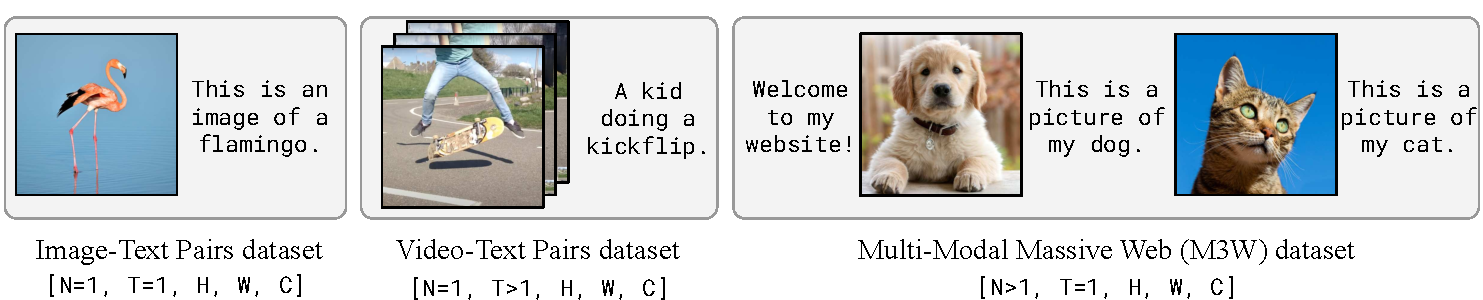
\includegraphics[width=\linewidth]{figures/fig0_data_mixture.pdf}
\centering
\caption{\small \textbf{Training datasets.} Mixture of training datasets of different formats. $N$ corresponds to the number of visual inputs for a single example. For paired image (or video) and text datasets, $N = 1$. $T$ is the number of video frames ($T = 1$ for images). $H$, $W$, and $C$ are height, width and color channels.}
\label{fig:training_data}
\end{figure}

We train the Flamingo models on a carefully chosen mixture of datasets illustrated in Figure~\ref{fig:training_data} and described next.

\label{app:datasets}

\subsubsection{\mmmw{} collection}
\label{app:collection-m3w}

The selection and scraping of web pages for \mmmw~follows a similar process to the one used for collecting the \emph{MassiveWeb} dataset~\citep{gopher}. We start by filtering out non-English documents. 
We also remove those that do not pass internal filters,
which identify explicit content across images, videos, and text. We use a custom scraper to extract salient content from the remaining documents, in the form of plain text interleaved with images, as described in Section \maintoappref{sec:interleaved_datasets}.
The text in \mmmw{} is collected in a similar fashion to that of \emph{MassiveWeb},
but we also collect any images present at the same level in the HTML tree. We discard documents for which the scraping process does not yield any images.

We then apply similar text filtering heuristics, to remove low quality documents and reduce repetition, as well as some image filters to remove images that are too small (either width or height less than 64 pixels), too wide or narrow (aspect ratio greater than 3 in either direction), or unambiguously low quality (e.g. single-colour images). We discard documents that no longer contain any images following this filtering step.

\subsubsection{\mmmw{} image-placement augmentation}
\label{app:m3w_processing}
\label{app:interleaved_indices}

During evaluation of \methodfamily{}, we prompt the model with an image and ask it to generate text for that image.
This lends itself to a natural sequencing at inference time in which the image comes before the corresponding text output.

However, the correspondence between images and text in our interleaved M3W dataset (Section~\maintoappref{sec:interleaved_datasets}) is in general unknown (and potentially not well-defined in certain cases).
As a motivating example, a simple webpage might be structured in either of the following ways:
\begin{enumerate}
    \item[(a)] This is my dog! <dog image> \hspace{1cm} This is my cat! <cat image>
    \item[(b)] <dog image> That was my dog! \hspace{1cm} <cat image> That was my cat!
\end{enumerate}
The text-aligned image indices (\texttt{indices}) might ``ideally'' be chosen such that at each point in the text, the index points to the most semantically relevant image for that text -- i.e., the next image in example (a), and the previous image in example (b).
In the absence of a general way to determine semantic correspondence between text and images on webpages ``in the wild'', we make a simplifying assumption that the most relevant image at any given point in the text is either the last image appearing before the text token, or the image immediately following it (as in the simple examples above), and choose \texttt{indices} accordingly.

During training, for each webpage sampled, we sample with probability $p_{next} = \frac{1}{2}$ whether \texttt{indices} are chosen to map text to the previous or next image.
This inevitably means we make the semantically ``unnatural'' choice -- e.g., associating the text ``This is my cat!'' with the dog image in (a) above -- around half of the time.
We ablate this choice in Section~\maintoappref{sec:ablations}, finding a small advantage to setting $p_{next} = \frac{1}{2}$ over either $0$ (always  the previous image index) or $1$ (always the next image index).
This suggests that there may be a beneficial ``data augmentation'' effect to this randomisation.



\subsubsection{\shortimagetextpairs{} and \shortvideotextpairs{}: Visual data paired with text}
\label{app:vtp_and_itp}

Along with our interleaved image and text dataset, we use several paired vision and text web datasets for training.
One dataset is ALIGN~\citep{align}, composed of 1.8 billion images paired with alt-text.
ALIGN is large, but noisy and limited to images.
The images are often poorly described by the corresponding alt-text annotation.
For this reason, we augment it with two datasets: \shortimagetextpairs{} (\imagetextpairs) consists of 312 million images, and \shortvideotextpairs{} (\videotextpairs) consists of 27 million short videos (approximately 22 seconds on average). Both datasets are paired with more descriptive captions.
For instance, the average number of tokens of an ALIGN text description is 12.4 per image, while it is 20.5 for the \shortimagetextpairs{} dataset.
The \shortimagetextpairs{} and \shortvideotextpairs{} datasets were collected by crawling fewer than ten websites targeting high-quality and rich image descriptions.
These single-image and single-video datasets are preprocessed analogously to the \mmmw{} data preprocessing described previously, adding the \texttt{<image>} tag at the beginning of the sequence (immediately after \texttt{<BOS>}), and the \texttt{<EOC>} token after the text (before \texttt{<EOS>}).
We deduplicated these datasets against all our benchmarks (against both the training and the evaluation sets) using image similarity, as detailed in Appendix~\ref{app:dataset_dedup}.
Datasheets for \shortimagetextpairs{} and \shortvideotextpairs{} are respectively given in Appendix~\ref{app:itp_datasheet} and Appendix~\ref{app:vtp_datasheet}.

\subsubsection{Dataset deduplication against evaluation tasks}
\label{app:dataset_dedup}

We used an internal deduplication tool to deduplicate our training datasets from our evaluation datasets.
This deduplication pipeline relies on a trained visual encoder which maps embedding closer together when they are potential duplicates.
Once the image embeddings have been computed, a fast approximate nearest neighbor search is performed on the training images to retrieve duplicate candidates from the validation datasets.
For the paired image-text dataset, we have deduplicated our \shortimagetextpairs{} and ALIGN training images against: ImageNet (train, val), COCO (train, valid, test), OK-VQA (train, valid, test), VQAv2 (train, valid, test), Flickr30k (train, valid, test), VisDial (train, valid, test).

We did not deduplicate our image datasets against VizWiz, HatefulMemes and TextVQA as we performed these evaluations only after having trained our \method{} models.
However, we believe this had no impact on our results as the images from these datasets are unlikely to be scraped from the web; VizWiz images were obtained using a specific mobile app and only available for download, HatefulMemes memes were created by researchers instead of being scraped on the web and finally TextVQA images are from OpenImages.

Note that we did not run the deduplication on the \mmmw{} dataset as one training example is a full webpage of interleaved paragraph with several images, unlikely to contain images from our benchmark suite.
To verify this hypothesis, we have obtained near-duplicate statistics on the 185M individual images from \mmmw{} and the results are the following: in total, 1314 potential duplicates were found from the validation and test splits of ImageNet, COCO, OK-VQA, VQAv2, Flickr30k and VisDial. Out of the 1314 candidates, only 125 are exact duplicates.

For the video datasets, we did not perform any deduplication of VTP (27M videos) as none of the collected VTP videos were obtained from YouTube or Flickr, which are the sources of all of our video evaluation datasets collected on the Internet.


